\documentclass[conference]{IEEEtran}

\usepackage{graphicx}
\usepackage{booktabs}
\usepackage{amsmath}
\usepackage{amssymb}
\usepackage{array}
\usepackage{url}
\usepackage[hidelinks]{hyperref}
\usepackage{pgfplots}
\pgfplotsset{compat=1.18}
\usepackage{xcolor}

\definecolor{ringcolor}{HTML}{00897B}
\definecolor{naivecolor}{HTML}{C1631A}

\begin{document}

\title{All-Reduce Strategies for Distributed Matrix Multiplication:\\
A Comparative Study on the Akita/MGPUSim Simulator}

\author{
\IEEEauthorblockN{Hamed Alinezhad}
\IEEEauthorblockA{
Department of Computer Engineering\\
Sharif University of Technology\\
Tehran, Iran\\
\textit{Supervised by Prof.\ Hamid Sarbazi-Azad}\\
Summer 2026}
}

\maketitle

\begin{abstract}
All-Reduce is the standard primitive for combining partial results computed independently across accelerators, and its communication cost often decides whether a multi-GPU workload scales at all. We implement a Naive (centralized) All-Reduce alongside the existing Ring All-Reduce in MGPUSim's \texttt{mccl} library, and integrate both into a contraction-dimension-split (K-split) distributed GEMM benchmark, in which All-Reduce is the genuine synchronization step rather than an incidental one. Across a sweep over matrix size, GPU count, and algorithm, Ring consistently outperforms Naive, with the gap widening as problem size and GPU count grow, while scaling efficiency for both algorithms falls sharply at 4 GPUs because communication cost does not shrink with $K$-splitting. A complementary cache/DRAM sensitivity study shows the benchmark is insensitive to L1 capacity, mildly sensitive to L2, and most sensitive to DRAM capacity, through reduced memory-controller parallelism rather than working-set overflow.
\end{abstract}

\begin{IEEEkeywords}
All-Reduce, collective communication, distributed GEMM, GPU simulation, MGPUSim, Akita
\end{IEEEkeywords}

\section{Introduction and Background}
\label{sec:intro}

All-Reduce is a collective operation in which $n$ participants, each holding a local array, combine their arrays with an associative operator (typically sum or average) so that every participant ends up holding the identical, fully reduced result. It is the standard way to synchronize partial results computed independently across workers -- for example, averaging gradients across replicas in distributed deep learning~\cite{patarasuk2009}, or, as studied here, summing partial matrix products computed on disjoint slices of a shared contraction dimension. Its communication volume is fixed by the size of the reduced array and does not shrink as more workers are added, so the choice of algorithm determines whether adding workers helps or hurts overall throughput.

\textbf{Ring All-Reduce}~\cite{patarasuk2009} arranges the $n$ participants in a ring and splits the array into $n$ chunks. A \emph{reduce-scatter} phase of $n-1$ steps has each participant forward one chunk to its successor while accumulating a chunk from its predecessor, leaving every participant holding one fully-reduced chunk; an \emph{all-gather} phase of $n-1$ further steps circulates those reduced chunks so every participant ends with the complete result. Every link carries the same amount of data at every step, so total bandwidth demand is spread evenly and no single link bottlenecks -- this is why Ring underlies most large-scale collective-communication libraries (e.g., NCCL) and its simulator analogue, \texttt{mccl}.

\textbf{Naive (centralized) All-Reduce} instead designates one participant as root: every other participant sends its data to the root, the root reduces the incoming data sequentially, and the root sends the final result back out to everyone. Every element of data crosses the root's link twice, so the root's bandwidth becomes an $O(n)$ bottleneck as $n$ grows, unlike Ring's evenly-distributed, $O(1)$-per-link cost. Naive serves here as the baseline against which Ring is evaluated.

Both algorithms are evaluated as the synchronization step of a distributed GEMM benchmark that splits the contraction ($K$) dimension across GPUs. Unlike an output-split GEMM, where combining per-GPU results is a simple gather of disjoint tiles, a $K$-split produces \emph{overlapping, full-size} partial products on every GPU that must be summed elementwise, making All-Reduce the genuine, load-bearing synchronization primitive rather than an artifact of the benchmark's structure.

\section{Implementation}
\label{sec:implementation}

We extend MGPUSim (built on the Akita discrete-event engine, modeling an AMD GCN3 R9 Nano GPU) in three ways. First, \texttt{AllReduceNaive} was added to \texttt{mccl} with the same signature as the existing \texttt{AllReduceRing}, so the two are interchangeable at call sites: it gathers every non-root GPU's chunk into the root, reduces (averaging) it there, then pushes the result back out directly to every other GPU. It reuses the same push/reduce GCN3 kernels as Ring, so the two algorithms differ only in communication pattern, making the comparison controlled.

Second, we built a K-split distributed GEMM benchmark: for $C = A \times B$, $A \in \mathbb{R}^{M \times K}$, $B \in \mathbb{R}^{K \times N}$, splitting $K$ evenly across $g$ GPUs gives each GPU a private $M \times (K/g)$ slice of $A$ and $(K/g) \times N$ slice of $B$, from which it computes a full-size $M \times N$ partial product using the existing tiled GCN3 matrix-multiplication kernel. The $g$ partial products are then combined via All-Reduce (Ring or Naive, selectable) over the flattened $M \times N$ array; since \texttt{mccl}'s reduction kernel averages rather than sums, the benchmark rescales the final result by $g$.

Third, we wired an L1 cache size knob and a working DRAM size knob into the \texttt{samples/runner} platform layer for the sensitivity study of Section~\ref{sec:results}; the DRAM knob had previously been silently disconnected from the GPU builder. Along the way we also worked around three latent simulator issues unrelated to this study's contributions: a broken kernel row-offset parameter (worked around with direct pointer-arithmetic addressing), a driver deadlock with multiple simultaneously-undrained command queues (worked around with round-robin, one-launch-per-GPU-per-round scheduling), and a DRAM-controller crash below $\sim$2\,GB capacity. All reported results were validated against a CPU reference implementation.

\section{Results and Evaluation}
\label{sec:results}

All experiments use MGPUSim's timing-accurate mode with the default R9 Nano configuration (64 CUs per GPU). The scaling sweep covers three cubic matrix sizes ($128^3$, $256^3$, $512^3$), three GPU counts (1, 2, 4), and both algorithms, at the default 16\,KB L1 / 2\,MB L2 / 4\,GB DRAM configuration. The sensitivity sweep fixes a $256^3$, 2-GPU, Ring workload and varies one parameter at a time.

Table~\ref{tab:scaling} and Figure~\ref{fig:scaling} show the representative $256^3$ case; the same pattern holds at $128^3$ and $512^3$. Ring is faster than Naive in every configuration tested, with the gap widening from 3\% at 1 GPU to 8--23\% at 4 GPUs as matrix size grows, consistent with Naive's root bandwidth becoming an $O(n)$ bottleneck against Ring's flatter cost. Scaling efficiency, however, is poor for \emph{both} algorithms, falling to 10--17\% at 4 GPUs regardless of matrix size: All-Reduce's communication volume is proportional to $M \times N$ and does not shrink as $K$ is split across more GPUs, so beyond a point adding GPUs actively hurts efficiency -- a standard "strong-scaling wall," reproduced here in a controlled simulator setting.

\begin{table}[htbp]
\caption{$256^3$ GEMM: speedup and efficiency relative to 1 GPU}
\label{tab:scaling}
\centering
\footnotesize
\begin{tabular}{@{}llrrr@{}}
\toprule
Alg. & GPUs & Time ($\mu$s) & Speedup & Efficiency \\
\midrule
Ring  & 1 & 991.6  & 1.000$\times$ & 100.0\% \\
Ring  & 2 & 1013.2 & 0.979$\times$ & 48.9\% \\
Ring  & 4 & 1493.0 & 0.664$\times$ & 16.6\% \\
Naive & 1 & 1010.5 & 1.000$\times$ & 100.0\% \\
Naive & 2 & 1128.4 & 0.896$\times$ & 44.8\% \\
Naive & 4 & 1845.2 & 0.548$\times$ & 13.7\% \\
\bottomrule
\end{tabular}
\end{table}

\begin{figure}[htbp]
\centering
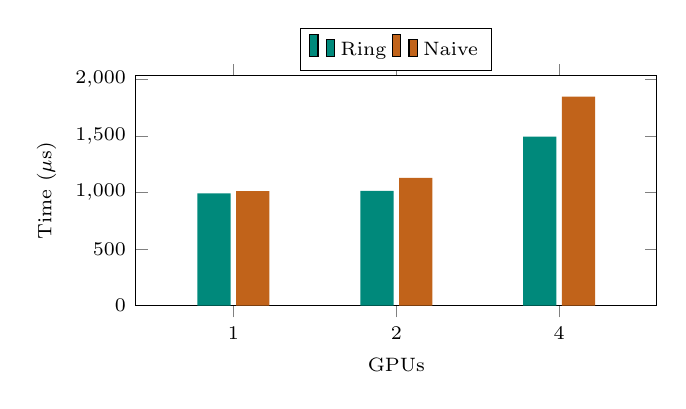
\begin{tikzpicture}
\begin{axis}[
  width=8.2cm, height=4.5cm,
  ybar, bar width=12pt,
  ymin=0,
  ylabel={Time ($\mu$s)},
  xlabel={GPUs},
  symbolic x coords={1,2,4},
  xtick=data,
  enlarge x limits=0.3,
  legend style={font=\scriptsize, at={(0.5,1.02)}, anchor=south, legend columns=-1},
  tick label style={font=\scriptsize},
  label style={font=\scriptsize},
]
\addplot[fill=ringcolor,draw=none] coordinates {(1,991.6) (2,1013.2) (4,1493.0)};
\addplot[fill=naivecolor,draw=none] coordinates {(1,1010.5) (2,1128.4) (4,1845.2)};
\legend{Ring, Naive}
\end{axis}
\end{tikzpicture}
\caption{Execution time vs.\ GPU count for $256^3$ GEMM.}
\label{fig:scaling}
\end{figure}

Table~\ref{tab:cache} shows the cache/DRAM sensitivity results. L1 capacity has essentially no effect ($\pm1.6\%$) across an $8\times$ range, consistent with the reused kernel caching its working tile in explicit local memory rather than relying on the hardware L1 -- its read-hit rate is 0\% at every size tested. L2 capacity has a small effect: halving it to 512\,KB costs 0.4\%. DRAM capacity dominates: restricting it to 2\,GB costs 22.1\%, even though L2 hit rate does not degrade -- ruling out working-set overflow. The cause is instead reduced DRAM rank-level parallelism at lower capacity, which lowers the memory controller's ability to hide access latency; this effect is confined to the GEMM kernel's own compute time and does not touch the All-Reduce phase, since DRAM capacity has no bearing on inter-GPU message passing.

\begin{table}[htbp]
\caption{Cache/DRAM sensitivity ($256^3$, 2 GPUs, Ring)}
\label{tab:cache}
\centering
\footnotesize
\begin{tabular}{@{}lrr@{}}
\toprule
Configuration & Time ($\mu$s) & $\Delta$ vs.\ baseline \\
\midrule
Baseline (16K/2M/4G) & 1013.3 & --- \\
L1 = 8KB  & 1029.4 & +1.6\% \\
L1 = 32KB & 1013.2 & $-$0.0\% \\
L2 = 512KB & 1017.5 & +0.4\% \\
L2 = 4MB  & 1013.2 & $-$0.0\% \\
DRAM = 2GB & 1237.7 & +22.1\% \\
\bottomrule
\end{tabular}
\end{table}

\section{Conclusion}
\label{sec:conclusion}

Ring All-Reduce consistently outperforms the centralized Naive baseline in a K-split distributed GEMM benchmark, with the advantage growing as problem size and GPU count increase, directly reflecting the two algorithms' communication topologies. Scaling efficiency nonetheless falls sharply for both algorithms at higher GPU counts, because All-Reduce's communication volume is fixed by output size and does not shrink with $K$-splitting -- the benchmark is communication-bound at the sizes tested. An architectural sensitivity study further shows this workload is insensitive to L1 capacity, mildly sensitive to L2, and most sensitive to DRAM capacity, acting through memory-controller parallelism rather than working-set capacity. Together, these results characterize both the algorithmic trade-off between All-Reduce strategies and the architectural sensitivities of a representative distributed-GEMM workload on a cycle-level multi-GPU simulator.

\begin{thebibliography}{9}

\bibitem{patarasuk2009}
P.~Patarasuk and X.~Yuan, ``Bandwidth optimal all-reduce algorithms for clusters of workstations,'' \emph{Journal of Parallel and Distributed Computing}, vol.~69, no.~2, pp.~117--124, 2009.

\bibitem{mgpusim2019}
Y.~Sun, T.~Baruah, S.~A.~Mojumder, S.~Dong, X.~Gong, S.~Treadway, Y.~Bao, S.~Hance, C.~McCardwell, V.~Zhao, H.~Barclay, A.~K.~Ziabari, Z.~Chen, R.~Ubal, J.~L.~Abell\'{a}n, J.~Kim, A.~Joshi, and D.~Kaeli, ``MGPUSim: Enabling multi-GPU performance modeling and optimization,'' in \emph{Proceedings of the 46th International Symposium on Computer Architecture (ISCA)}, 2019, pp.~197--209.

\end{thebibliography}

\end{document}
